\chapter{The Results Manager}

\subsection{Generating Indicators}
Once the simulation is finished, which should not take long since the initial configuration only runs for one year, you can explore the results in the Results Manager.  Click on the Results Manager tab, and expand the model.gridcell entry under Indicator\_libraries.You will see some initial indicators that are available.  Right-click on the population indicator and select \emph{Generate results with}.  The screen should now show a new frame on the right that has pull-down menus to configure and compute this indicator, shown in Figure \ref{fig:opus-generate-indicator}.  The initial indicator is a population by gridcell indicator, which requires computing the number of persons in each household that are located in buildings that are located in gridcells.  This particular example uses a variable to do this computation.  Variables are coded as very small Python programs.  An alternative, simpler approach to use is the Opus Expression Language, which has been recently created to make available to non-programmers much of the power of doing complex calculations such as this, with a simple syntax.  This is covered in the documentation, and later in this chapter. 

\begin{figure}[htp]
\begin{center}
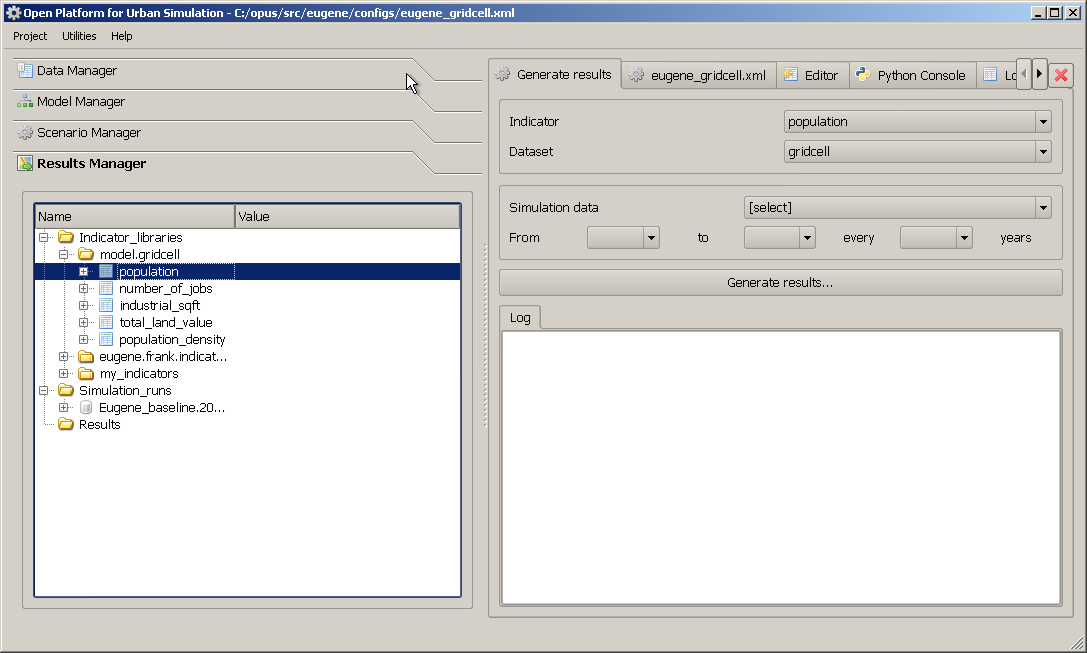
\includegraphics[scale=0.4]{graphics/opus-generate-indicator.png}
\end{center}
\caption{Generating an Indicator in the Results Manager}
\label{fig:opus-generate-indicator}
\end{figure}

You will need to click the \verb#Simulation data# button and then select the simulation results you want to use.  Notice that the name of the scenario contains a date and time when the run was started.  Once you click on the \verb#Generate results# button, the indicator is computed.  A message is printed to the log, below the button, and a new entry will show up in the results node in the Results Manager tab on the left, as shown in Figure \ref{fig:opus-indicator-2}.

\begin{figure}[htp]
\begin{center}
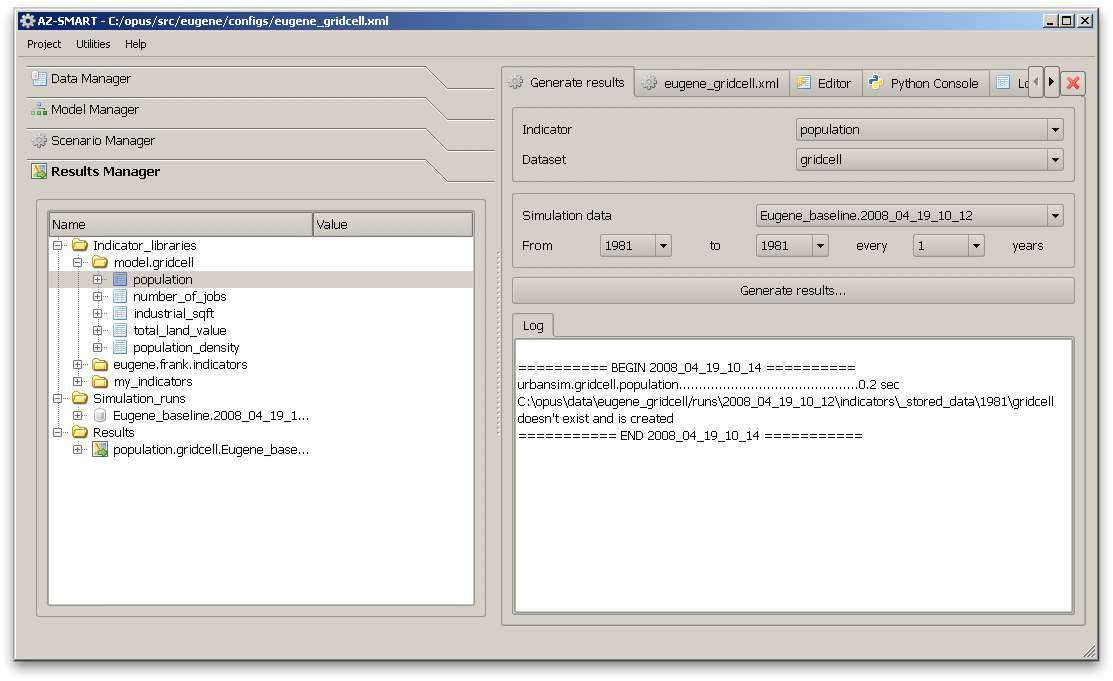
\includegraphics[scale=0.4]{graphics/opus-indicator-2.png}
\end{center}
\caption{Result of Generating an Indicator}
\label{fig:opus-indicator-2}
\end{figure}

Now that an indicator has been computed, its data is available to visualize or export to another application.  The Results Manager currently supports several ways to visualize an indicator, and these will depend on the nature of the indicator.  The menu for this is shown in Figure \ref{fig:opus-indicator-view-1}.  For example, the indicator that has just been computed is population by gridcell.  It is possible to visualize data on a grid using a simple image map, displayed on the right hand window using the Matplotlib Python library.   If you select the Map (Matplotlib) option on the menu, it will generate a map such as the one shown in Figure \ref{fig:opus-indicator-view-2}.

\begin{figure}[htp]
\begin{center}
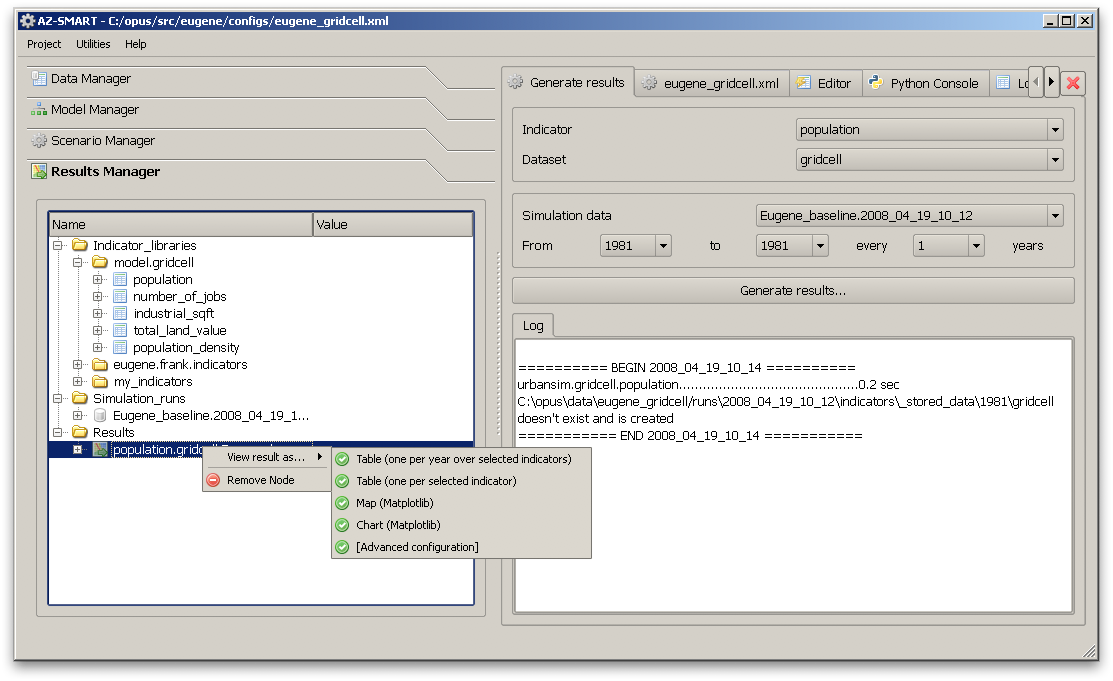
\includegraphics[scale=0.4]{graphics/opus-indicator-view-1.png}
\end{center}
\caption{View Results for an Indicator}
\label{fig:opus-indicator-view-1}
\end{figure}

\begin{figure}[htp]
\begin{center}
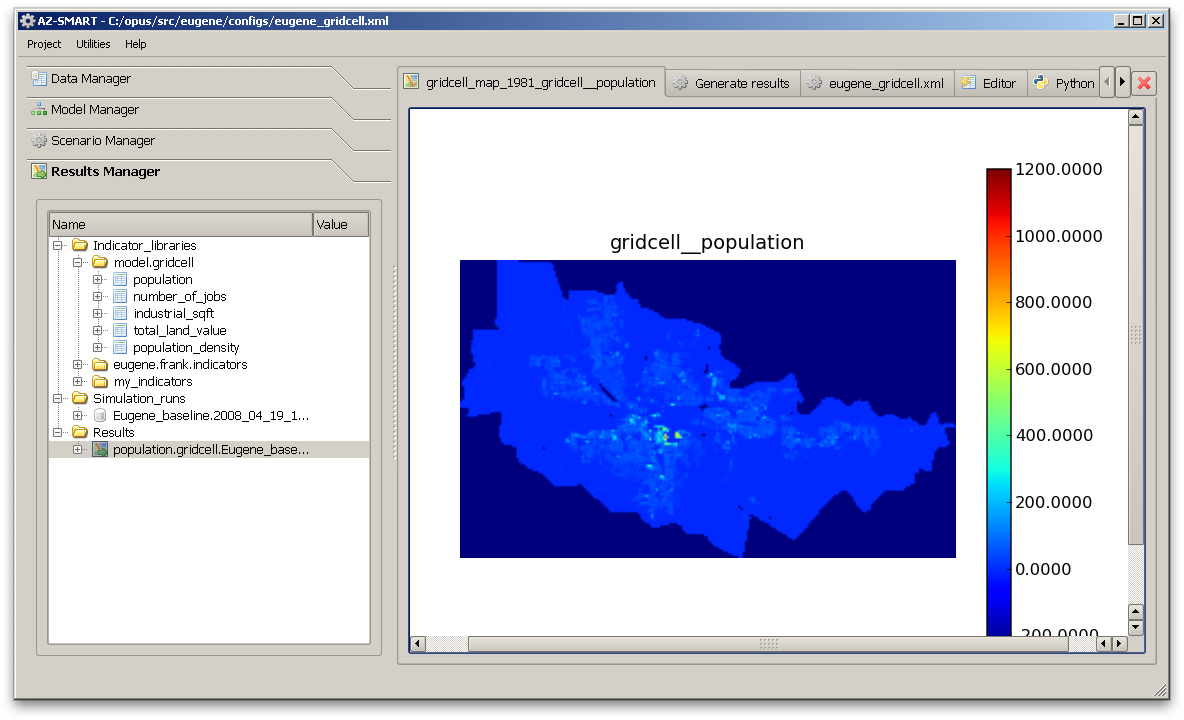
\includegraphics[scale=0.4]{graphics/opus-indicator-view-2.png}
\end{center}
\caption{Matplotlib Map for Population by Gridcell in Eugene-Springfield in 1981}
\label{fig:opus-indicator-view-2}
\end{figure}

The Matplotlib map is not intended to replace GIS-based mapping, which allows far more control and the overlay of other features for visual reference.  It is merely a quick tool to visualize data to get a sense of the spatial patterns in it.  In order to support visualization in a GIS environment such as ArcGIS or QGIS, the results may be exported to a database or geodatabase environment, and the GIS software used to create a more interactive and flexible display of the data.

